\documentclass[border=1cm]{standalone}

\usepackage{tikz}

\begin{document}
    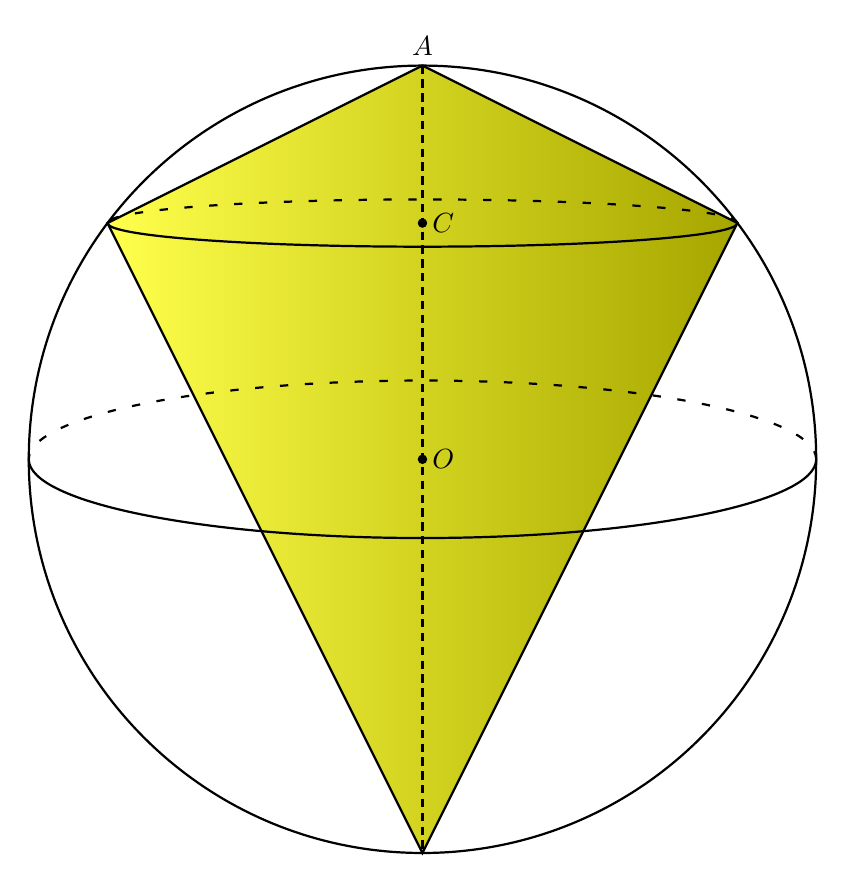
\begin{tikzpicture}
        \coordinate[label=right:{$O$}] (O) at (0,0);
        \coordinate[label=above:{$A$}] (A) at (0,5);
        \coordinate (B) at (0,-5);
        \coordinate (C) at (0,3);

        \draw[thick, left color = yellow!70,right color = olive!70] (A)--(-4,3)--(B)--(4,3)--cycle;

        \draw[thick] (O) circle [radius=5];
        \draw[thick] (-5, 0) arc [start angle=-180, end angle=0, x radius=5cm, y radius=1cm];
        \draw[thick, loosely dashed] (5, 0) arc [start angle=0, end angle=180, x radius=5cm, y radius=1cm];
        
        \draw[thick] (-4, 3) arc [start angle=-180, end angle=0, x radius=4cm, y radius=0.3cm];
        \draw[thick, loosely dashed] (4, 3) arc [start angle=0, end angle=180, x radius=4cm, y radius=0.3cm];
        
        \draw[thick,densely dashed](A)--(B);
        \draw[fill] (O) circle [radius=1.5pt];
        \draw[fill] (C) circle [radius=1.5pt];
        \node[right] at (C) {$C$};
        \node[right] at (O) {$O$};

    \end{tikzpicture}
\end{document}